\documentclass{beamer}
\usetheme{Warsaw}

\usepackage[utf8]{inputenc}
\usepackage{fancybox}
\usepackage{multimedia} 
\usepackage{subfig}
\usepackage{amsmath}
\usepackage{hyperref}
\usepackage[all]{xy}
\begin{document}


\title[Angewandte Mathematik] % (optional, only for long titles)
{Angewandte Mathematik
\\
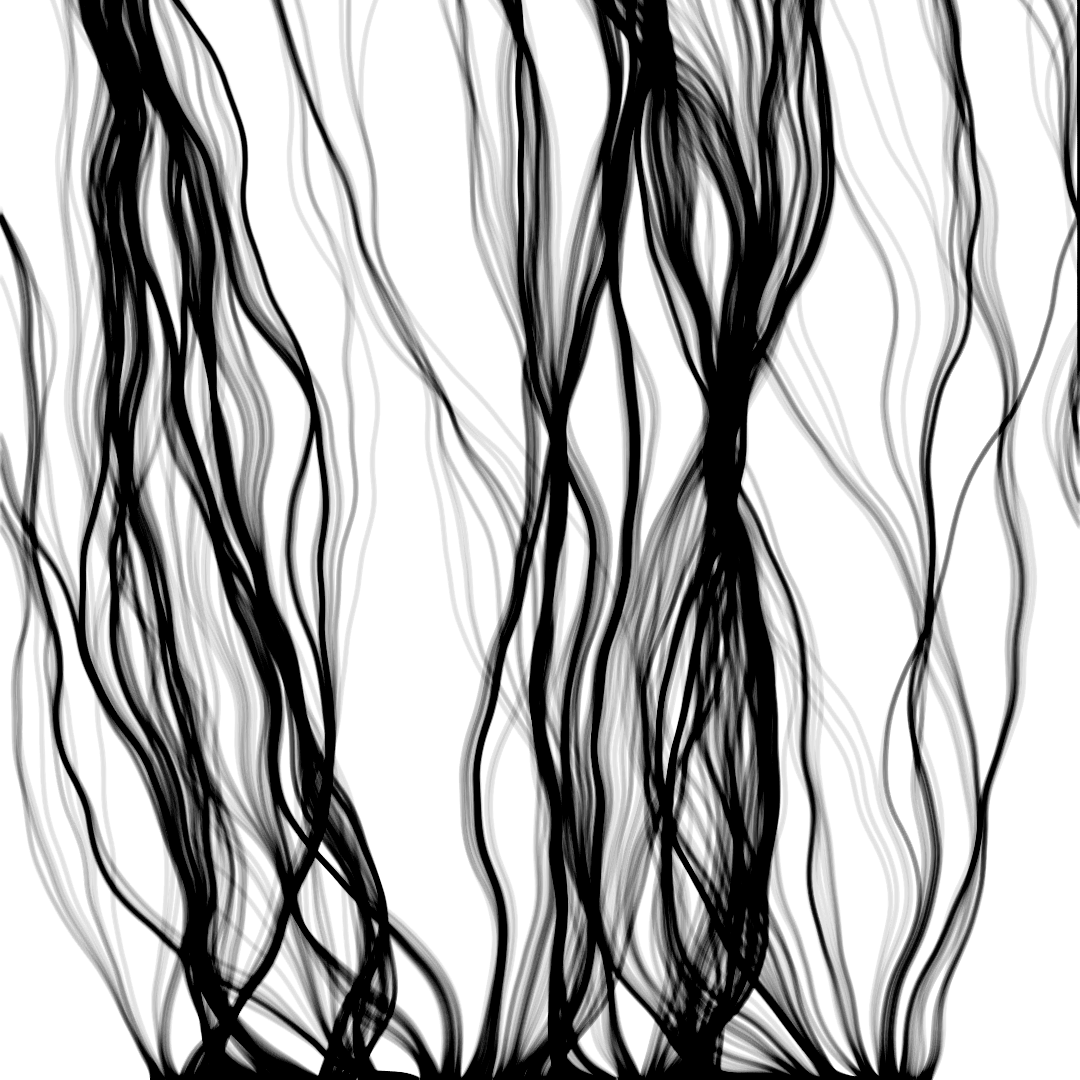
\includegraphics[scale=0.15]{images/cover}
}
\subtitle{}
\author[Dr. Johannes Riesterer] % (optional, for multiple authors)
{Dr.  rer. nat. Johannes Riesterer}

\date[KPT 2004] % (optional)
{}

\subject{Angewandte Mathematik}



\begin{frame}
    \frametitle{Mehrdimensionale Differentialrechnung}
\framesubtitle{Limes}
    \begin{block}{Konvergenz}
Sei $f :X \subset \mathbb{R}^n \to \mathbb{R}^m$ eine  Funktion und $a \in X$. Wir nennen $L_a \in \mathbb{R}^m$ Grenzwert von $f$ bezüglich der Annäherung von $x$ an $a$, falls für jede  konvergente Folge $x_n \to a$  die Folge $f(x_n)$ nach $L_a$ konvergiert.  In diesem Fall bezeichnen wir
\begin{align*}
\lim_{x \to a} f(x) = L_a \;.
\end{align*}
Dies ist gleichbedeutend damit, dass für jedes $\epsilon > 0$ ein $\delta > 0$ existiert, so dass
$d(f(x) ,L_a) < \epsilon$ gilt für jedes $x$ mit $d(x, a) < \delta$.
\end{block}

 \end{frame}


\begin{frame}
    \frametitle{Mehrdimensionale Differentialrechnung}
\framesubtitle{Limes}
    \begin{block}{Stetigkeit}
Eine reellwertige Funktion $f :U \to \mathbb{R}$ heißt stetig, wenn für alle $y \in U$ der Grenzwert $\lim_{x \to y} f(x) = L_{y} $ existiert.

\end{block}

 \end{frame}

\begin{frame}
    \frametitle{Mehrdimensionale Differentialrechnung}
\framesubtitle{Limes}

\begin{figure}[H]
      \centering
    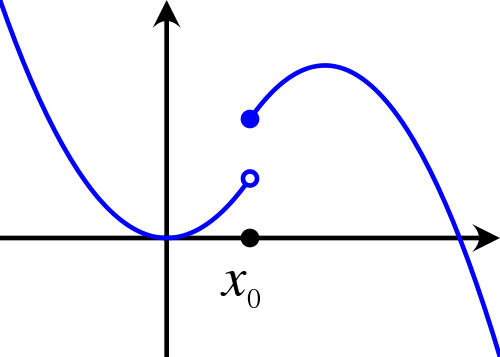
\includegraphics[width=0.8\textwidth]{images/500px-Upper_semi}
      \caption{Quelle: Wikipedia: https://commons.wikimedia.org/wiki/File:Upper\_semi.svg}
\end{figure}

 \end{frame}

\begin{frame}
    \frametitle{Mehrdimensionale Differentialrechnung}
\framesubtitle{Limes}
    \begin{block}{Landau Notation}
Für eine Funktion $g : U \subset \mathbb{R}^n \to \mathbb{R}$ bezeichnen wir die Wachstumsklasse 
\begin{align*}
o(g) := \{ f : U  \to \mathbb{R} \; | \; \lim_{x \to a} \frac {|f(x)|}{|g(x)|} = 0 \; \forall a \in U \} \\
O(g) := \{ f : U  \to \mathbb{R} \; | \; \lim_{x \to a} \frac {|f(x)|}{|g(x)|} < \infty \; \forall a \in U \}
\end{align*}
\end{block}
 \end{frame}


\begin{frame}
    \frametitle{Angewandte Mathematik}
\framesubtitle{Lokale Linearisierung}
    \begin{block}{Lokale Linearisierung}
Eine Funktion  $f: U \subset \mathbb{R}^n \to \mathbb{R}$ heisst differenzierter  in $a \in U$ falls es eine lineare Funktion 
$df(a):  \mathbb{R}^n \to  \mathbb{R}^n$ gibt mit
\begin{align}
\label{diff}
f(a + h)  =  f(a)  +  df(a)  h + o(||h||) 
\end{align}
für alle $h \in \mathbb{R}^n$
\end{block}
    \begin{block}{Bedeutung}
Eine differenzierbare Funktion kann  auf hinreichend kleinen Umgebungen 
beliebig genau durch eine lineare Funktion approximiert werden. 
\end{block}
 \end{frame}

\begin{frame}
    \frametitle{Mehrdimensionale Differentialrechnung}
\framesubtitle{Limes}

\begin{figure}[H]
      \centering
    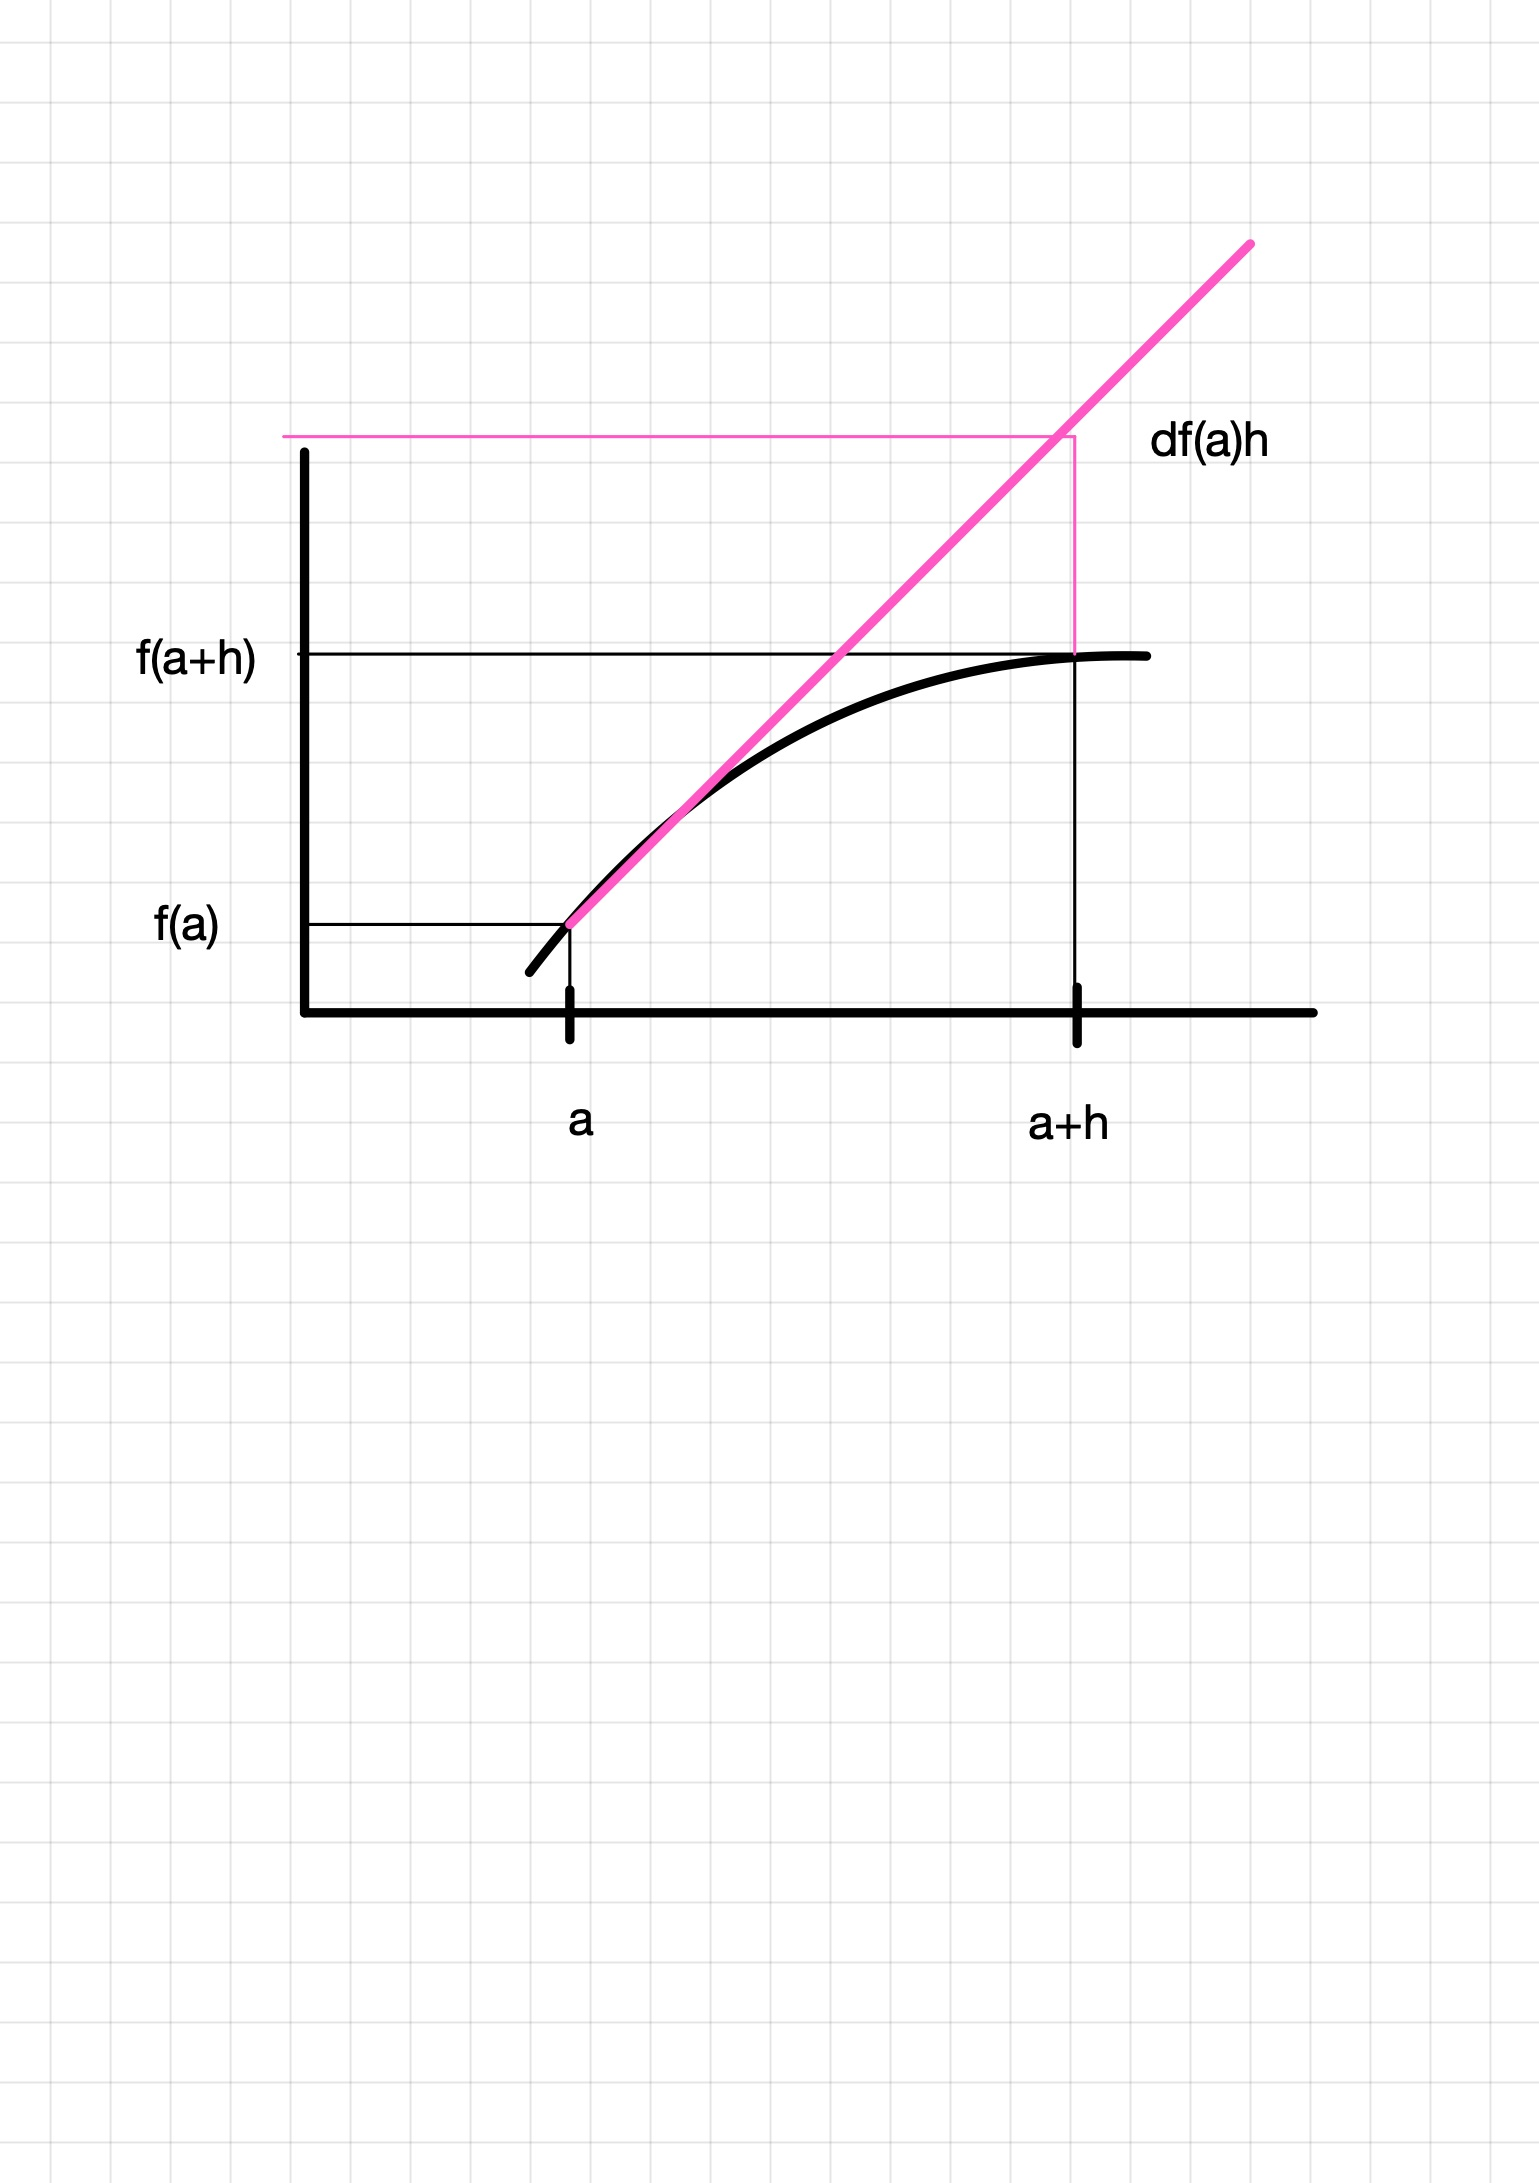
\includegraphics[width=0.8\textwidth]{images/df}
\end{figure}

 \end{frame}



\begin{frame}
    \frametitle{Mehrdimensionale Differentialrechnung}
\framesubtitle{Limes}
    \begin{block}{Eindeutigkeit}
Die lineare Abbildung $df(a)$ ist eindeutig bestimmt.
\end{block}
    \begin{block}{Beweis}
Ist $df'(a)$ eine weiter Abbildung mit Eigenschaft $(\ref{diff})$, so gilt für jeden Basisvektor $e_i$
\begin{align}
(df(a) - df'(a))(e_i) = lim_{t \to 0}\frac{(df'(a) - df(a))(t e_i)}{||te_i||} = 0
\end{align}
\end{block}
 \end{frame}


\begin{frame}
    \frametitle{Mehrdimensionale Differentialrechnung}
\framesubtitle{Limes}
    \begin{block}{Beispiel}
\begin{align}
f(x) : = A\cdot x + b \\
df(a) : = A 
\end{align}
\end{block}
    \begin{block}{Beweis}
\begin{align}
& \lim_{h\to 0} \frac{A(x + h) - A\cdot x -A\cdot h}{||h||} = \\
& \lim_{h\to 0} \frac{A\cdot x + A \cdot h - A\cdot x -A\cdot h}{||h||} = 0
\end{align}
\end{block}

 \end{frame}



\begin{frame}
    \frametitle{Mehrdimensionale Differentialrechnung}
\framesubtitle{Limes}
    \begin{block}{Ableitung}
Ist $f$ differenzierter in $U$, so gilt wegen der Linearität 
\begin{align}
df(a)h = \sum_{i= 1}^n (df(a)e_i)\cdot h_i
\end{align}
wobei $(e_1, \cdots, e_n)$ die Standardbasis des $\mathbb{R}^n$ ist.
Die einzeilige Matrix
\begin{align}
f'(a) := (df(a) e_1, \cdots ,  df(a) e_n)
\end{align}
heißt Ableitung von $f$ in $a$.
\end{block}

 \end{frame}



\begin{frame}
    \frametitle{Mehrdimensionale Differentialrechnung}
\framesubtitle{Differenzierbarkeit}
    \begin{block}{Richtungsableitung}
Sei $f: U \to \mathbb{R}$ eine Funktion. Für einen Vektor $h \in  \mathbb{R}^n$  und einen Punkt  $a \in U$ heißt der Grenzwert (falls er existiert) 
\begin{align*}
\partial_h f(a) := \lim_{t \to 0} \frac{f(a + th) - f(a)}{t}
\end{align*}
Richtungsableitung von $f$ am Punkt $a$ in Richtung $h$. Sie misst die Änderung der Funktion in Richtung $h$.

Speziell nennen wir für die Standard Basisvektoren $e_i$ 
\begin{align*}
\frac{\partial f(a)}{\partial x_n}  := \partial_{e_i} f(a) := \lim_{t \to 0} \frac{f(a + t e_i) - f(a)}{t}
\end{align*}
die partielle Ableitung von $f$ in $a$ nach $x_i$.
\end{block}


 \end{frame}



\begin{frame}
    \frametitle{Mehrdimensionale Differentialrechnung}
\framesubtitle{Limes}

\begin{figure}[H]
      \centering
    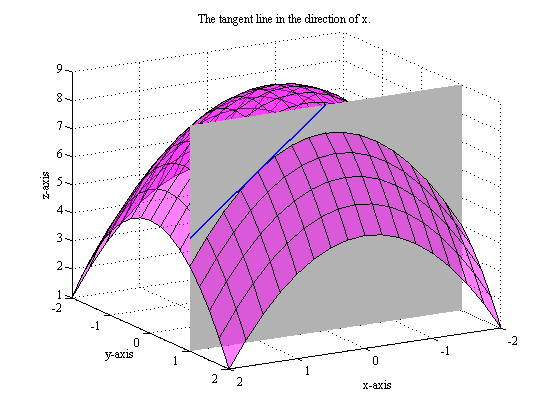
\includegraphics[width=0.8\textwidth]{images/diffable}
\end{figure}

 \end{frame}

\begin{frame}
    \frametitle{Mehrdimensionale Differentialrechnung}
\framesubtitle{Differenzierbarkeit}
    \begin{block}{Partielle Differenzierbarkeit }
Eine Funktion  $f: U \to \mathbb{R}$ heißt partiell differenzierbar im Punkt $a \in U$, falls alle partiellen Ableitungen 
$$\frac{\partial f(a)}{\partial x_1}, \cdots , \frac{\partial f(a)}{\partial x_n}$$ 
existieren.
\end{block}
 \end{frame}



\begin{frame}
    \frametitle{Mehrdimensionale Differentialrechnung}
\framesubtitle{Differenzierbarkeit}
    \begin{block}{Beispiel}

\end{block}
 \end{frame}

\begin{frame}
    \frametitle{Mehrdimensionale Differentialrechnung}
\framesubtitle{Differenzierbarkeit}
    \begin{block}{Beispiel}
Ist eine Funktion $f$ in $a$ differenzierter, so ist sie dort partiell differenzierbar und es gilt
\begin{align*}
df(a)h = f'(a)h = \sum_{i=1}^{n} \partial_i f(a) \cdot h_i \\
f'(a) = \bigl( \partial_1f(a), \cdots , \partial_n f(a) \bigr)
\end{align*}

\end{block}
 \end{frame}

\begin{frame}
    \frametitle{Mehrdimensionale Differentialrechnung}
\framesubtitle{Differenzierbarkeit}
    \begin{block}{Beweis}
Ist $f$ differenzierter, so gilt für $t \in \mathbb{R}$ und $h \in \mathbb{R}^n$
\begin{align*}
& f(a + th)  =  f(a)  +  df(a) th + R(||th||) \\
& \lim_{h \to 0} \frac{|R(th)|}{|th|} = 0 \\
&\Rightarrow  \lim_{t \to 0} \frac{|R(th)|}{|th|} = 0 \\
&\Rightarrow  df(a)h = \lim_{t \to 0} \frac{f(a+th) - f(a)}{|t|} = \partial_h f(a)\\
&\Rightarrow df(a)e_i = \partial_if(a)
\end{align*}
\end{block}

 \end{frame}



\begin{frame}
    \frametitle{Mehrdimensionale Differentialrechnung}
\framesubtitle{Differenzierbarkeit}
    \begin{block}{Differenzierbarkeis Kriterium}
Eine Funktion $f: U \to \mathbb{R}$ ist  differenzierbar im Punkt $a \in U$, falls alle partiellen Ableitungen 
$$\frac{\partial f(a)}{\partial x_1}, \cdots, \frac{\partial f(a)}{\partial x_n}$$
 existieren und stetig sind.  
\end{block}
 \end{frame}


\begin{frame}
    \frametitle{Mehrdimensionale Differentialrechnung}
\framesubtitle{Vorwissen über eindimensionale  Funktionen}
    \begin{block}{Mittelwertsatz einer Veränderlichen}
Sei $f : [a,b] \to \mathbb{R}$ stetig und differenzierbar für alle $x \in (a,b)$. Dann gibt es $\xi \in (a,b)$ mit
$f'(\xi) = \frac{f(b) - f(a)} { b-a}$.
\end{block}
\begin{figure}[H]
      \centering
    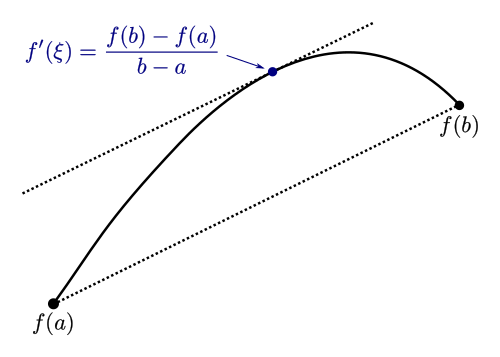
\includegraphics[width=0.5\textwidth]{images/Mittelwertsatz3.png}
      \caption{Quelle: Wikipedia: https://commons.wikimedia.org/wiki/File:Mittelwertsatz3.svg}
\end{figure}
 \end{frame}



\begin{frame}
    \frametitle{Angewandte Mathematik}
\framesubtitle{Lokale Linearisierung}
    \begin{block}{Beweis}
\begin{figure}[H]
      \centering
    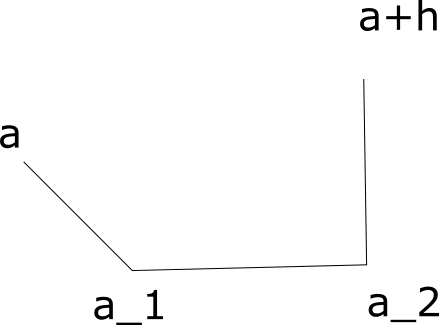
\includegraphics[width=0.4\textwidth]{images/kantenzug}
      \caption{Kantenzug mit achesenparallelen Kanten}
\end{figure}

\end{block}
    \begin{block}{Beweis}

\begin{align*}
& a_0 := a \\
& a_i  := a_{i-1} + h_i e_i;  \;  \;  i = 1, \cdots , n
\end{align*} 
\end{block}

 \end{frame}




\begin{frame}
    \frametitle{Angewandte Mathematik}
\framesubtitle{Lokale Linearisierung}
    \begin{block}{Beweis}
\begin{itemize}
\item $f(a + h) - f(a) = \sum_{i=1}^{n} \bigl( f (a_i)   - f(a_{i-1})   \bigr)$
\pause \item  Mit $\varphi_i(t) : = f(a_i + t e_i)$ gilt  $f(a_i) - f(a_{i-1}) = \varphi_i(h_i)  - \varphi_i(0)$
\pause \item Mittelwertsatz einer Veränderlichen:  Es gibt  $\tau_i$  mit
\begin{align*}
\varphi_i(h_i)  - \varphi_i(0)  = h_i \varphi'(\tau_i) \;.
\end{align*}
\pause \item 
\begin{align*}
f(a + h) - f(a) - df(a) \cdot h = \sum_{i=1}^n  \biggl( \frac{\partial  f(\xi) }{\partial x_i} -    \frac{\partial  f(a) }{\partial x_i}   \biggr) h_i
\end{align*} 
\end {itemize}

 
Da $\varphi'_i(t) = \frac{\partial  f(a_{i-1} + t e_i ) }{\partial x_i}$ und mit $\xi_i: = a_i + \tau_i e_i$ 
\end{block}

 \end{frame}

\begin{frame}
    \frametitle{Angewandte Mathematik}
\framesubtitle{Lokale Linearisierung}
    \begin{block}{Beweis}
\begin{align*}
| f(a + h) - f(a) - df(a) \cdot h |  \leq || h ||_{\infty}  \sum_{i=1}^n  \biggl| \frac{\partial  f(\xi) }{\partial x_i} -    \frac{\partial  f(a) }{\partial x_i}   \biggr | \; . 
\end{align*} 
Für $h \to 0$ gilt $\xi_i \to a$ und da die partiellen Ableitung stetig sind nach Voraussetzung und alle Normen äquivalent sind folgt

\begin{align*}
\lim_{h \to 0} \frac{ f(a + h) - f(a) - df(a) \cdot h}{||h||} = 0 
\end{align*} 

\end{block}

 \end{frame}



\begin{frame}
    \frametitle{Angewandte Mathematik}
\framesubtitle{Differential}
    \begin{block}{Eigenschaften des Differentials}
Für das Differential einer differenzierbaren Funktion  $f: U \to \mathbb{R}$ gilt für alle $a \in U$:
\begin{itemize}
\item $df(a)  \cdot h = \partial_h f(a)$. 
\item $d (f \cdot g)(a) = g df(a) + f(a) dg$
\item $d(f + g)(a) = df(a) + dg(a)$
\end{itemize}
\end{block}
 \end{frame}

\begin{frame}
    \frametitle{Angewandte Mathematik}
\framesubtitle{Differential}
    \begin{block}{Beweis}
\begin{itemize}
\item Für die Basisvektoren ist per Definition $df(a)  \cdot e_i = \partial_{e_i} f(a)$. Da jeder Vektor $h$ eine Linearkombination der Basisvektoren ist und $df$ linear ist, folgt die Behauptung.
\item Folgt direkt aus der entsprechenden Eigenschaft reeller Funktionen.
\item Folgt direkt aus der entsprechenden Eigenschaft reeller Funktionen.
\end{itemize}
\end{block}
 \end{frame}




\begin{frame}
    \frametitle{Mehrdimensionale Differentialrechnung}
\framesubtitle{Differenzierbarkeit}
    \begin{block}{Gradient}

Der Vektor 
$$\nabla f (a) := \begin{pmatrix}  \frac{\partial f(a)}{\partial x_1} \\  \vdots \\ \frac{\partial f(a)}{\partial x_n}  \end{pmatrix}$$
wird als Gradient bezeichnet. Es ist $df(a) \cdot h = \langle \nabla f (a) , h \rangle$.
\end{block}
\begin{figure}[H]
      \centering
    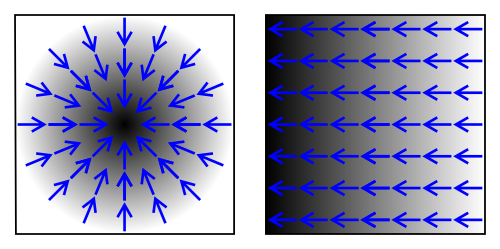
\includegraphics[width=0.7\textwidth]{images/Gradient}
      \caption{Quelle: Wikipedia: https://commons.wikimedia.org/wiki/File:Gradient2.svg}
\end{figure}


 \end{frame}


\begin{frame}
    \frametitle{Mehrdimensionale Differentialrechnung}
\framesubtitle{Differenzierbarkeit}
    \begin{block}{Gradient}

Sei   $f: U \to \mathbb{R}$ differenzierbare Funktion,  $a \in U$ und $v := \text{argmax}_{ ||h|| = 1 } \{ \partial_h f(a) \}$.
Dann gilt 
\begin{align*}
|| \nabla f(a) || v =  \nabla f(a) \; .
\end{align*} 
\end{block}
\begin{block}{Gradient}
Der Gradient zeigt in die Richtung des steilsten Anstiegs.
\end{block}

 \end{frame}

\begin{frame}
    \frametitle{Mehrdimensionale Differentialrechnung}
\framesubtitle{Differenzierbarkeit}
    \begin{block}{Beweis}
Für beliebiges $h$ gilt 
\begin{align*}
\partial_h f(a) = df(a) h = \langle \nabla f(a) , h \rangle = || \nabla f(a)||  \cdot ||h|| \cdot \cos(\varphi) 
\end{align*} 
wobei $\varphi$ den Innenwinkel zwischen $\nabla f(a)$ und $h$ bezeichnet. Für $||h|| = 1$ wird somit $\partial_h f(a) $ maximal, wenn $\varphi = 0$ und somit$h =  \frac{\nabla f(a)}{||\nabla f(a)||}$ ist.
\end{block}

 \end{frame}




\end{document}

